\documentclass[11pt,a4paper]{article}

\usepackage[margin=1in]{geometry}
\usepackage{titlesec}
\usepackage{enumitem}
\usepackage{hyperref}
\usepackage{parskip}
\usepackage{graphicx}
\usepackage{float}
\usepackage{booktabs}
\usepackage{amsmath}

\hypersetup{colorlinks=true, linkcolor=blue, urlcolor=blue}

\titleformat{\section}{\large\bfseries}{\thesection}{0.5em}{}
\titleformat{\subsection}{\normalsize\bfseries}{\thesubsection}{0.5em}{}
\setlist{leftmargin=1.4em, topsep=2pt, itemsep=2pt}

\title{\vspace{-1.5cm}\textbf{PKCERT AI \& Software Development Internship \\ Task 14: Ensemble Methods -- Bagging \& Boosting}}
\author{Abdullah Amir}
\date{AI and Software Development \\ 21 July 2026}

\begin{document}

\maketitle
\vspace{-0.8cm}

This report covers the theory and the results. The full code, outputs and plots live in
the notebook \texttt{ensemble\_methods.ipynb}. The dataset is the \textbf{UCI Bank
Marketing} dataset: 45,211 phone calls made by a Portuguese bank's telemarketing team to
sell term deposits, of which \textbf{11.7\% ended in a subscription}. A single Decision
Tree, a \textbf{Bagging} ensemble, and two \textbf{Boosting} implementations
(\textbf{XGBoost} and \textbf{LightGBM}) are compared on it.

% ----------------------------------------------------------------
\section*{Part A: Dataset Selection \& Preparation}

\textbf{What the features are.} Each row is one call. Seven numeric features
(\texttt{age}, \texttt{balance}, \texttt{day}, \texttt{duration}, \texttt{campaign},
\texttt{pdays}, \texttt{previous}) and nine categorical features (\texttt{job},
\texttt{marital}, \texttt{education}, \texttt{default}, \texttt{housing}, \texttt{loan},
\texttt{contact}, \texttt{month}, \texttt{poutcome}). The target \texttt{y} is whether the
client subscribed to a term deposit.

\textbf{Missing values and encoding.} There are no missing values -- categorical gaps are
already coded as an explicit \texttt{"unknown"} category, which is itself informative:
\texttt{poutcome} (outcome of the previous marketing contact) is \texttt{unknown} for 82\%
of clients, meaning most were never contacted before. Categoricals are one-hot encoded via
a \texttt{ColumnTransformer}; numeric columns pass through untouched, since tree-based
models are invariant to monotonic rescaling.

\textbf{Split.} An 80/20 train/test split, stratified on \texttt{y}: 4,231 subscriptions
in the 36,168-row training set, 1,058 in the 9,043-row test set.

\textbf{A leakage caveat, checked rather than ignored.} \texttt{duration} is the length of
the call \emph{itself}, which cannot be known before the call is placed -- a bank cannot
use it to decide whether to dial. UCI's own documentation flags this. Every score in this
report keeps \texttt{duration} in, the same choice almost every published benchmark on
this dataset makes, so every number here is an upper bound on what a real-time model could
achieve, not a real-time estimate.

\begin{figure}[H]
    \centering
    
\includegraphics[width=0.95\textwidth]{figures/01_dataset_overview.png}
    \caption{Left: the target is imbalanced, 11.7\% subscribed. Right: call duration by
    outcome -- successful calls run roughly 2.4x longer (median 426s vs 164s), which is
    exactly the leakage signal described above.}
\end{figure}

% ----------------------------------------------------------------
\section*{Part B: Bagging}

\textbf{What it is.} Bagging (Bootstrap Aggregating) trains many copies of the same base
learner, each on an independent bootstrap resample of the training data, and averages
their predictions. Averaging cancels out each tree's idiosyncratic mistakes without
requiring any single tree to be careful, so the base learner used here is an unpruned
Decision Tree, the same one used as the baseline in Part A.

\begin{table}[H]
\centering
\begin{tabular}{lrrrrr}
\toprule
\textbf{Model} & \textbf{Train Acc} & \textbf{Test Acc} & \textbf{Precision} & \textbf{Recall} & \textbf{ROC-AUC} \\
\midrule
Single Decision Tree & 1.0000 & 0.8746 & 0.4649 & 0.4754 & 0.7015 \\
Bagging (100 trees) & 1.0000 & 0.9055 & 0.6270 & 0.4735 & 0.9253 \\
\bottomrule
\end{tabular}
\caption{The single tree, and the bagged ensemble built from 100 copies of it.}
\end{table}

\begin{figure}[H]
    \centering
    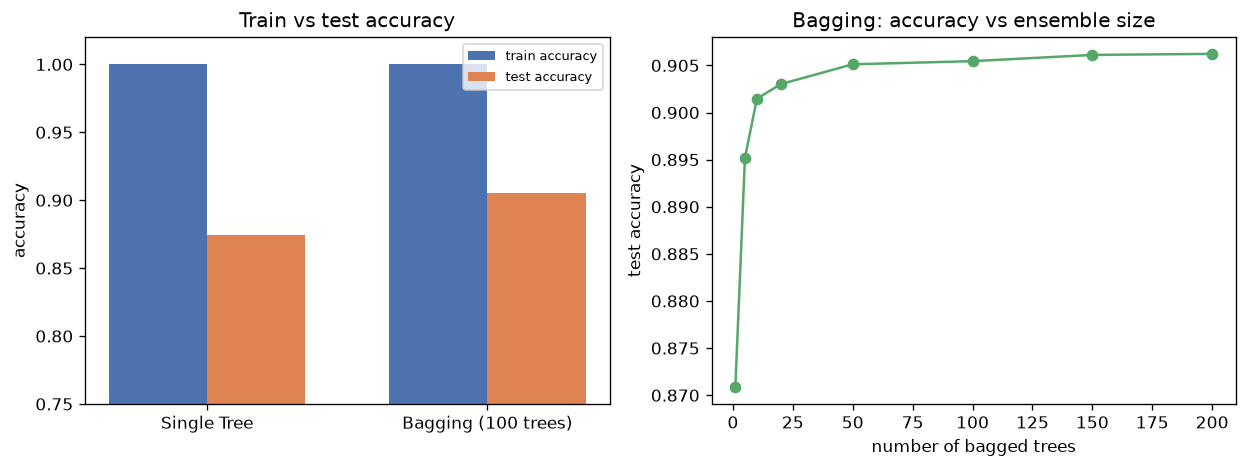
\includegraphics[width=0.95\textwidth]{figures/02_single_tree_vs_bagging.png}
    \caption{Left: train vs test accuracy for the single tree and the bagged ensemble.
    Right: bagging's test accuracy as more trees are added.}
\end{figure}

\textbf{The two panels together tell a specific, checkable story.} Bagging's
\emph{train} accuracy is still \textbf{1.0000} -- identical to the single tree. Bagging
does not stop the individual trees from memorising their own bootstrap sample; that is
not what it is for. What it fixes is \emph{test} accuracy, which rises from 0.8746 to
\textbf{0.9055}, and ROC-AUC, which rises from 0.7015 to \textbf{0.9253}, because
averaging cancels out each tree's individually wrong guesses on data it has not seen. The
out-of-bag estimate (0.9038) tracks the true test accuracy closely, confirming this is a
genuine generalisation gain and not an artefact of the particular test split. The right
panel shows the gain arrives fast: almost all of it is captured by 20--50 trees, and the
next 150 buy only a fraction of a percentage point.

\textbf{Advantages.} Reduces variance without increasing bias; trees train independently
so the method parallelises trivially across cores; the out-of-bag samples give a free
validation estimate without sacrificing any training data. \textbf{Limitations.} Does
nothing for the base learner's \emph{bias} -- bagging a shallow, weak tree would still
underfit; 100 full-depth trees are expensive to store and slow to train and predict with,
demonstrated concretely in Part D. \textbf{Use cases.} High-variance, low-bias base
learners (unpruned trees especially), and any setting where training can be
parallelised across independent workers with no sequential dependency.

% ----------------------------------------------------------------
\section*{Part C: Boosting}

\textbf{What it is.} Boosting trains trees \emph{sequentially}: each new tree fits the
errors the ensemble has made so far, rather than an independent bootstrap resample. Two
implementations were compared, both with shallow trees (\texttt{max\_depth=4}) and 300
boosting rounds.

\begin{table}[H]
\centering
\begin{tabular}{lrrrrr}
\toprule
\textbf{Model} & \textbf{Accuracy} & \textbf{Precision} & \textbf{Recall} & \textbf{F1} & \textbf{ROC-AUC} \\
\midrule
Bagging (100 trees) & 0.9055 & 0.6270 & 0.4735 & 0.5396 & 0.9253 \\
XGBoost & \textbf{0.9103} & \textbf{0.6631} & 0.4745 & \textbf{0.5532} & 0.9335 \\
LightGBM & 0.9090 & 0.6520 & \textbf{0.4764} & 0.5505 & \textbf{0.9339} \\
\bottomrule
\end{tabular}
\caption{Boosting against Bagging, same test set.}
\end{table}

\begin{figure}[H]
    \centering
    
\includegraphics[width=0.95\textwidth]{figures/03_confusion_matrices.png}
    \caption{Confusion matrices for all four models. Precision climbs steadily from the
    single tree (0.465) through bagging (0.627) to boosting (0.65--0.66); recall is
    essentially flat at 0.47--0.48 across every ensemble.}
\end{figure}

\begin{figure}[H]
    \centering
    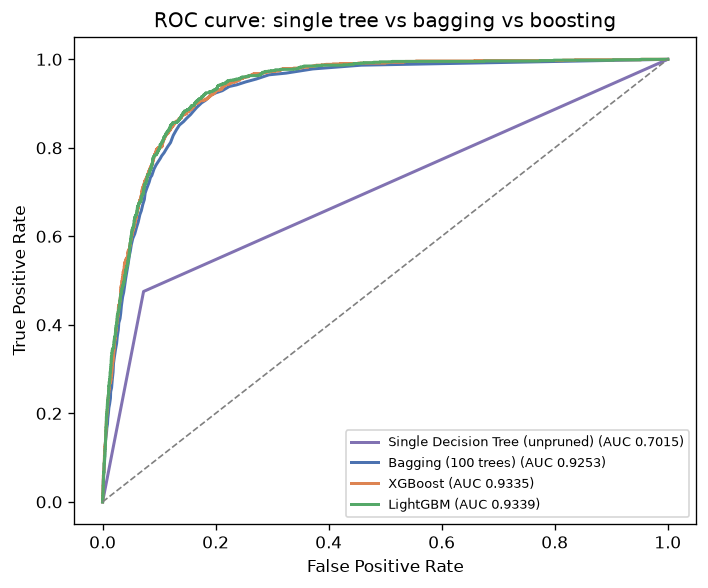
\includegraphics[width=0.68\textwidth]{figures/04_roc_comparison.png}
    \caption{ROC curves for all four models. Bagging and both boosting methods sit well
    above the single tree; XGBoost and LightGBM are visually indistinguishable from each
    other.}
\end{figure}

\textbf{Both boosting models beat bagging and the single tree on every metric}, and beat
\emph{each other} by a margin small enough to be noise: XGBoost edges ahead on accuracy,
precision and F1, LightGBM edges ahead on ROC-AUC by 0.0004. Neither result should be
read as one algorithm being fundamentally better than the other on this problem.

\begin{figure}[H]
    \centering
    
\includegraphics[width=0.72\textwidth]{figures/05_feature_importance.png}
    \caption{XGBoost's gain-based feature importance. \texttt{poutcome\_success} --
    whether this client said yes to a \emph{previous} campaign -- outranks even the
    leakage feature \texttt{duration}.}
\end{figure}

\textbf{The more interesting finding is not the score, it is what drives it.} The single
most important feature is \texttt{poutcome\_success}, ahead of \texttt{duration} itself:
past behaviour outpredicts even the leakage-prone call-length feature. \texttt{contact\_unknown} (no valid phone number on file) ranks second. Raw demographics like age and
balance do not make the top 12 at all.

\textbf{Advantages.} Highest accuracy of anything tried here, achieved with
\emph{shallower} trees than bagging needed. \textbf{Limitations.} Sequential by
construction, so unlike bagging it cannot be parallelised across trees; more
hyperparameters to tune (learning rate, tree depth, number of rounds) and more prone to
overfitting if over-tuned. \textbf{Applications.} The default choice for tabular data in
industry and in competitions, exactly the setting here.

% ----------------------------------------------------------------
\section*{Part D: Comparative Analysis \& Recommendation}

\begin{figure}[H]
    \centering
    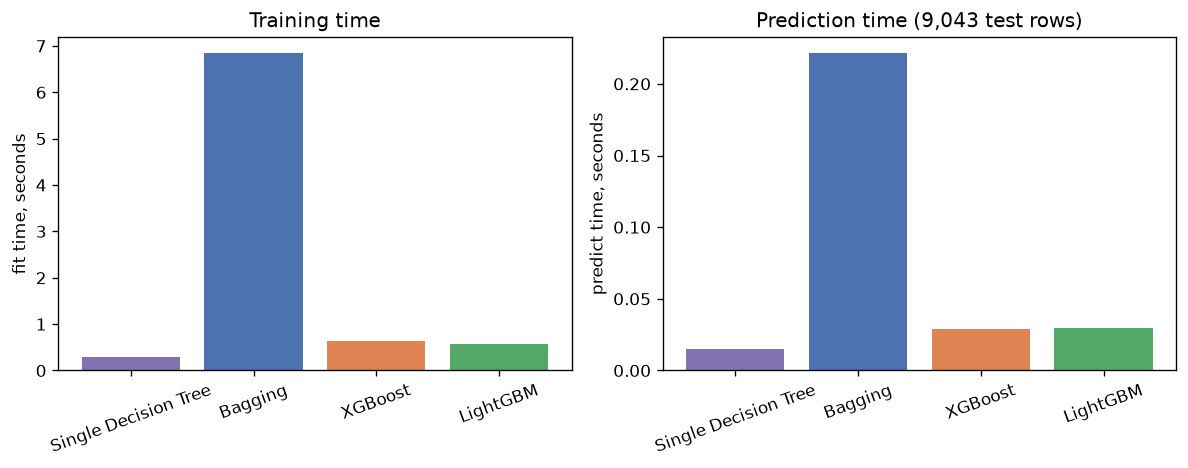
\includegraphics[width=0.95\textwidth]{figures/06_timing_comparison.png}
    \caption{Training and prediction time for all four models. Bagging is by far the
    slowest to train and to predict with, despite scoring lower than either boosting
    method.}
\end{figure}

\textbf{Performance.} Boosting (XGBoost 0.9103 accuracy / 0.9335 ROC-AUC, LightGBM 0.9090
/ 0.9339) beats Bagging (0.9055 / 0.9253), which beats the single tree (0.8746 / 0.7015),
consistently across accuracy, precision, F1 and ROC-AUC -- this is not an artefact of any
one metric.

\textbf{Computational efficiency, and this is the sharper result.} Bagging took
\textbf{6.85 seconds} to fit; XGBoost took \textbf{0.63s} and LightGBM \textbf{0.58s} --
boosting was \textbf{over 10x faster than bagging while also scoring higher}. This is not
a coincidence: bagging's 100 trees are each grown to full, unpruned depth, while
boosting's 300 trees are capped at depth 4. Shallow trees are cheap to build and to
evaluate, and sequential correction needs far fewer splits per tree than independent
bootstrap averaging does. Prediction time shows the same gap: 0.221s for bagging against
0.029s for XGBoost on the same 9,043 test rows.

\textbf{Recommendation.} For this dataset, \emph{boosting is the clear choice, either
XGBoost or LightGBM} -- the two are statistically indistinguishable here, with
LightGBM's histogram-based binning giving it a further small speed edge that would
compound on a larger dataset. Boosting beats bagging on every accuracy metric while
training more than 10x faster, and its shallow trees are cheaper to store and serve in
production. Bagging remains the right tool when the base learner's variance is the
whole problem and training must be distributed across independent workers with no
sequential dependency; it is not the right tool here, where a sequential method reached
a better answer for a fraction of the compute.

\textbf{The caveat that matters most.} \texttt{duration} is a leakage feature (Part A); a
bank that wanted to \emph{decide} whether to place a call, rather than evaluate calls
after the fact, would need to drop it, and every score in this report would fall.
Nothing about removing one feature is expected to favour bootstrap averaging over
sequential correction, so the \emph{ranking} between bagging and boosting should hold,
but the absolute numbers above should not be read as achievable in a real-time dialling
system.

\textbf{Conclusion.} The thread running through this task is that ensembling is not one
idea wearing two names. Bagging and boosting fix different problems: bagging cancels
variance in an already-low-bias, high-variance learner by averaging independent copies of
it; boosting reduces bias by having each new, deliberately weak learner correct the
ensemble's current mistakes. On a mixed tabular dataset like this one, with strong
signal concentrated in a handful of features, boosting's sequential correction found a
better answer with an order of magnitude less compute than bagging's brute-force
averaging -- and the reason why is visible in the tree depths each method needed to get
there.

\vspace{0.4cm}
\noindent The notebook and README are on GitHub: {\small\scalebox{0.72}[1]{\url{https://github.com/AbdullahAmir06/ai-internship-abdullahamir}}}

\end{document}
